\chapter[O Traveller Framework]{O Traveller Framework}

A proposta deste trabalho foi a construção de um \textit{framework} de definição de trajetórias para robôs móveis, mais especificamente, algoritmos globais de definição de trajetória. Foram implementados os quatro algoritmos descritos no capítulo 2 (Grafo de Visibilidade, Voronoi, Quadtree e Wavefront). Um mapa do ambiente é recebido da camada de mapeamento e o algoritmo cria um grafo a partir dele, definindo os caminhos livres que podem ser percorridos. Após isso, é executado um algoritmo de melhor caminho (como Djikstra ou A*, por exemplo) para definir o caminho a ser percorrido pelo robô. 

O núcleo do \textit{framework} roda em um computador fora do robô, como em um servidor local, e se comunica com o robô via comunicação \textit{bluetooth}. A escolha de desenvolver a solução fora da máquina será explicada no capítulo 6. No robô, uma classe encapsula a comunicação com o servidor e realiza a troca de mensagens. O servidor recebe os dados de entrada e opera os algoritmos para devolver ao robô a lista de pontos a serem percorridos.

A Figura 20 demonstra as tarefas principais do \textit{framework}, bem como suas entradas e saídas. Essas entradas e saídas definem como o \textit{framework} se comunica com as demais camadas do robô bem como as dependências desse framework para cumprir seu funcionamento. Cada tarefa apresentada representa um módulo do \textit{framework}, e as interações entre eles representa as estruturas de dados utilizadas para se comunicarem. Estes dados são recebidos pela classe embarcada no robô. Essa classe se comunica com o servidor. Os dados ainda são repassados para esse servidor sem alterações. Todo o processamento é então feito fora do robô, retornando uma resposta à classe embarcada. Por fim, essa classe responde ao sistema do robô.
 
\begin{figure}[h]
	\centering
	\label{fig20}
		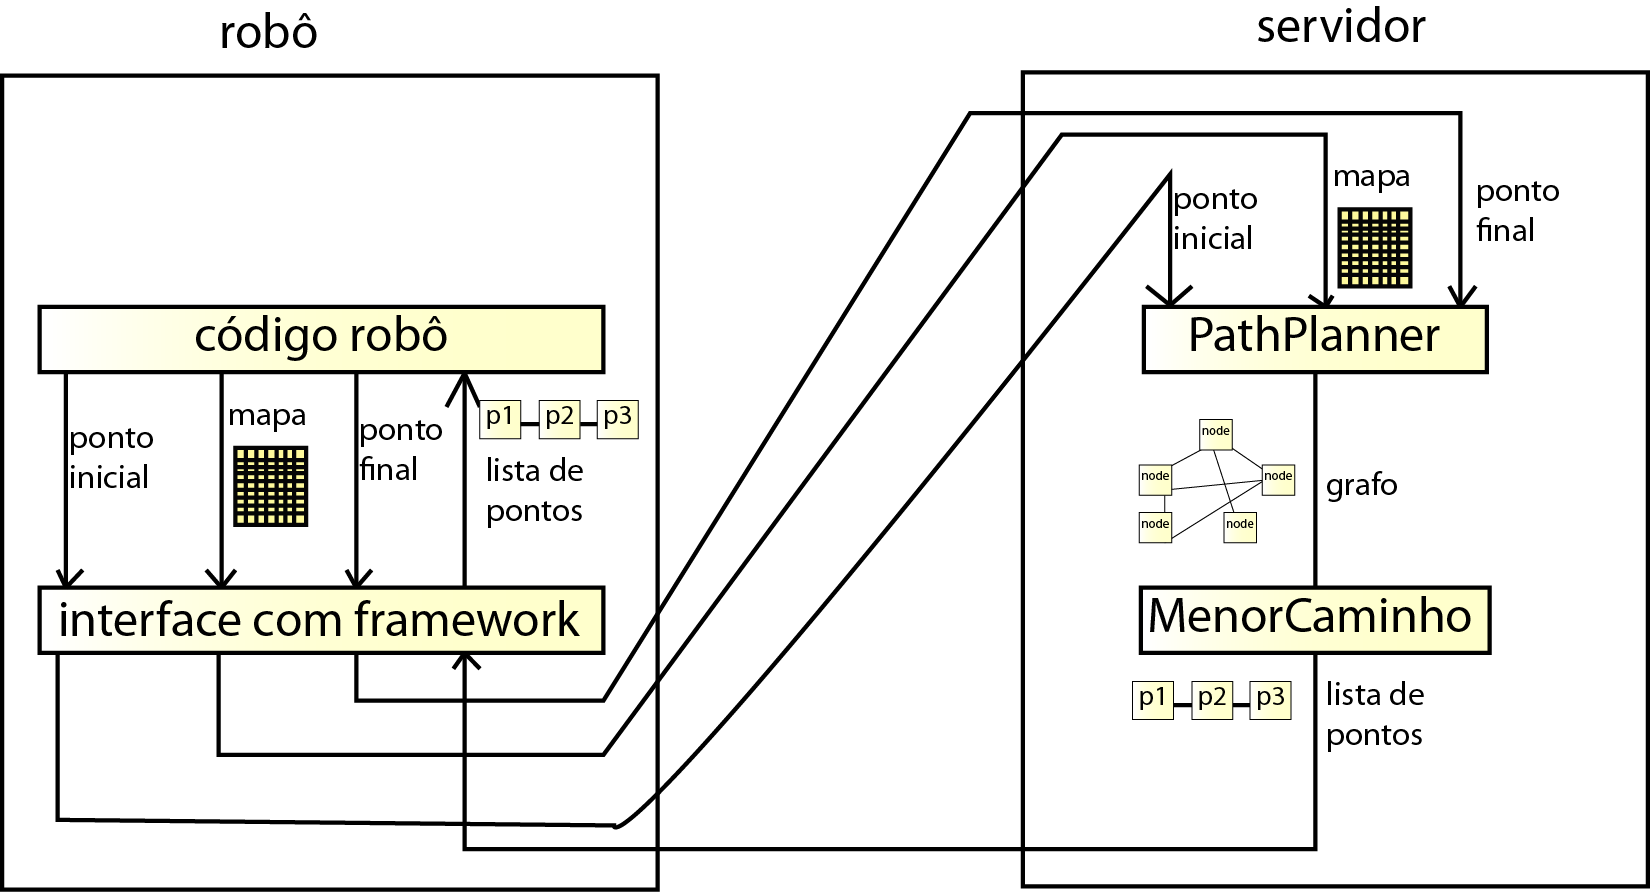
\includegraphics[keepaspectratio=true,scale=0.9]{figuras/framework.png}
	\caption{Estrutura do funcionamento do \textit{framework}}
\end{figure} 

A arquitetura geral do robô foi considerada como na Figura 21, orientada de acordo com a visão do autor \cite{Nehmzow2003}. Todas as abordagens da arquitetura de navegação seguiam uma lógica semelhante e apresentavam pequenas diferenças entre si. Assim sendo, esta estrutura mantêm as características apresentadas no capítulo 2.

\begin{figure}[h]
	\centering
	\label{fig21}
		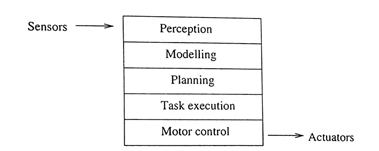
\includegraphics[keepaspectratio=true,scale=1]{figuras/arqusada.jpg}
	\caption{Arquitetura de navegação considerada, \cite{Nehmzow2003}}
\end{figure}

A definição de trajetória e o \textit{framework} participam da terceira camada. Como as camadas acima (\textit{Perception} e \textit{Modelling}) são responsáveis pelo mapeamento e entregam o mapa completo, os algoritmos globais e o Traveller Framework não precisam se preocupar com a comunicação com os sensores. As camadas abaixo (\textit{Task execution} e \textit{Motor control}) recebem a lista de coordenadas para onde o robô deve ir e cuidam do controle dos motores para chegar nesses pontos, considerando os graus de liberdade do robô (que varia de acordo com sua estrutura física). Assim, a camada a ser criada não se comunica nem com os sensores nem com os motores, o que confere a essa camada maior independência das configurações de robô. Baseado nessa abordagem, é esperado que o \textit{framework} funcione em variados tipos de robôs, não apenas no modelo \textit{differential steering} testado.

A seguir é definido como funciona em detalhes o Traveller e sua arquitetura.

\section{A Arquitetura}

A arquitetura de navegação costuma ser em camadas, como mostrado no capítulo 2.2.5. O Traveller trabalha dentro da camada de planejamento de trajetória e é uma estrutura baseada em componentes. Uma arquitetura em camadas dentro de outra poderia gerar indireções desnecessárias, além de uma abordagem por componentes suprir de forma mais adequada as necessidades do \textit{framework}.

Cada funcionalidade é efetuada por um componente diferente, projetado para consumir o mínimo de memória e depender o mínimo de outros componentes e de bibliotecas externas (incluindo as próprias do Java). Cada módulo tem a preocupação de ser o mais auto-suficiente possível, tendo apenas as interações necessárias para o seu funcionamento. Cada um dos módulos foi constantemente avaliado quanto a seu acoplamento, coesão,  simplicidade e facilidade de compreensão. Estas características serão melhor definidas na seção 5.6.

O \textit{framework} segue o padrão caixa-cinza, pois é desejável que o mesmo seja transparente e configurável pelo usuário. O usuário do \textit{framework} é livre para usar as implementações já prontas dos algoritmos de definição de trajetória e melhor caminho ou criar as suas próprias a partir das classes abstratas fornecidas. Além disso, o fluxo de execução e alguns comportamentos são mantidos estáticos.

O diagrama de componentes da Figura 22 mostra os módulos do \textit{framework} e suas interações. São apresentados os componentes conhecidos pelos outros componentes, mas não quais classes. Levando em conta o princípio de programar para interfaces, as classes conhecidas serão sempre as interfaces e classes abstratas (exceto nos compententes de estrutra de dados). Para simplificar o diagrama, as classes concretas foram retiradas, bem como foram criados diagramas específicos para detalhar cada módulo.

\begin{figure}[h]
	\centering
	\label{fig22}
		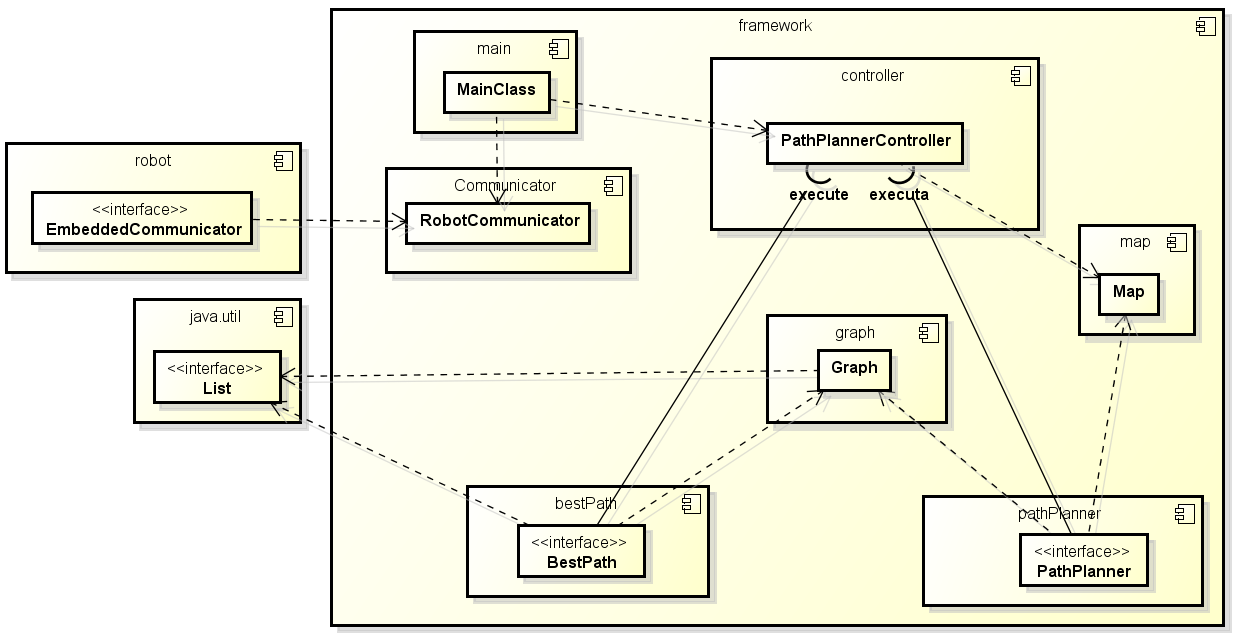
\includegraphics[keepaspectratio=true,scale=0.4]{figuras/componentes.png}
	\caption{Diagrama de pacotes do sistema}
\end{figure}

Nas seções subsequentes, cada componente é descrito detalhadamente.

\subsection{EmbeddedCommunicator}

\begin{figure}[h]
	\centering
	\label{fig23}
		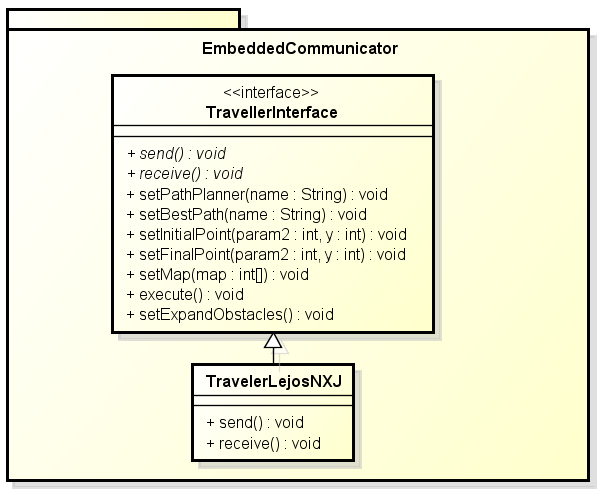
\includegraphics[keepaspectratio=true,scale=0.6]{figuras/embedded.png}
	\caption{Componente embarcado no robô}
\end{figure}

Este componente é o único que será executado dentro do robô e sua função é se comunicar com o servidor que esteja rodando o \textit{framework}, realizando as trocas de mensagens. Como cada kit possui uma programação, cada um pode realizar a comunicação externa de forma diferente. As classes e argumentos entre cada robô podem mudar, por isso é definida uma interface genérica de comunicação e uma classe concreta para o Lego NXT. A Figura 23 mostra a estrutura do pacote.

Na classe abstrata são implementados os métodos que recebem os dados do robô e que devolvem a lista para o mesmo, além de organizar as trocas de mensagens para o correto envio de informações. Essa classe abstrata define o padrão de troca de informações através do padrão de projeto Template, estabelecendo a ordem em que as mensagens devem ser enviadas, porém não define como o método \textit{send} e \textit{receive} funcionam. Esses métodos são definidos pela classe filha, que deve ser construída pelo usuário de acordo com as bibliotecas do kit que utiliza.

As únicas restrições feitas pela interface são: (i) que a comunicação seja \textit{bluetooth} para que o servidor consiga receber os dados, e (ii) que possam ser enviados \textit{strings} e \textit{arrays} de inteiros e booleanos pelo kit.

\subsection{RobotCommunicator}

\begin{figure}[h]
	\centering
	\label{fig24}
		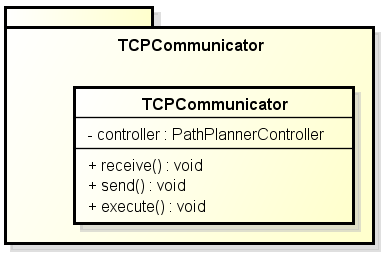
\includegraphics[keepaspectratio=true,scale=0.6]{figuras/tcp.png}
	\caption{Componente que se comunica com o robô}
\end{figure}

Este módulo apenas recebe os dados do robô e os repassa para o módulo controlador, que é o responsável pelo processamento desses dados. Esse módulo apenas separa o funcionamento de ambos, controlador e parte web. Assim, qualquer alteração na forma de comunicação ou na ordem da troca de informação não impactará no \textit{framework}. Este módulo também reorganiza os dados do mapa em uma nova matriz de booleanos para então repassá-los ao controlador. A Figura 24 mostra as principais funções do módulo.

\subsection{Controller}

\begin{figure}[h]
	\centering
	\label{fig25}
		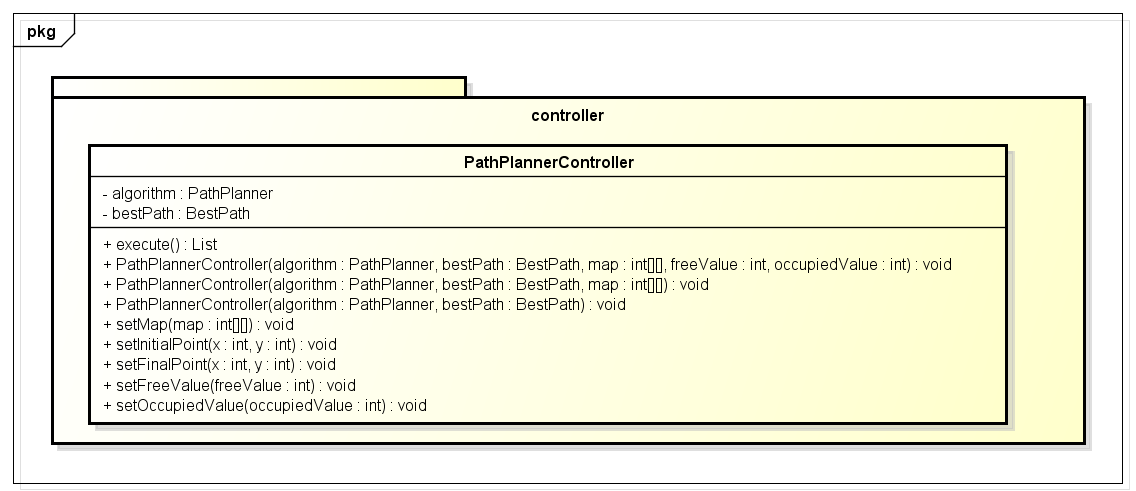
\includegraphics[keepaspectratio=true,scale=0.6]{figuras/pkgcontroller.png}
	\caption{Componente Controller}
\end{figure}

Uma vez recebidos os dados do robô pela camada RobotCommunicator, a classe PathPlannerController tem como propósito executar o \textit{framework} em si. Essa classe controla o fluxo de trabalho da aplicação, chamando os métodos das demais classes na ordem, e verificando seu correto funcionamento.

O componente segue os princípios Controlador e Inversão de Controle. Em vez do usuário chamar todas as funções do componente e fazer seu controle diretamente toda vez que quiser definir uma trajetória, este componente realiza esta tarefa pelo usuário, diminuindo acoplamento entre o usuário e o subsistema. A Inversão de Controle está presente pelo usuário ser o responsável por definir quais as classes dos outros componentes. Embora o \textit{framework} as instancie, cabe ao usuário escolher quais de suas variações serão implementadas. No construtor da classe, são passados os objetos PathPlanner e BestPath a serem usados. Esses objetos são armazenados e utilizados no método \textit{execute} para calcular o percurso. Isso permite ao módulo não conhecer as variações de cada interface, desacoplando-o dos demais módulos.

Os padrões utilizados são o Fachada e a Injeção de Dependência.

É também atribuído a esse módulo a responsabilidade por criar a estrutura local do mapa. O controlador inicializa o mapa, definindo os pontos inciais e finais. Adicionalmente, limpa a memória ao final do procedimento, delegando ao componente PathPlanner apenas a tarefa de utilizar o mapa.

O diagrama de sequência apresentado na seção 2.4 mostrou de forma bastante superficial o funcionamento do sistema para dar uma visão geral das funcionalidades e sequência de ações. O diagrama na Figura 26 demonstra de forma mais aprofundada como realmente é feito o trabalho do framework, com foco no componente controller.

\begin{figure}[h]
	\centering
	\label{fig26}
		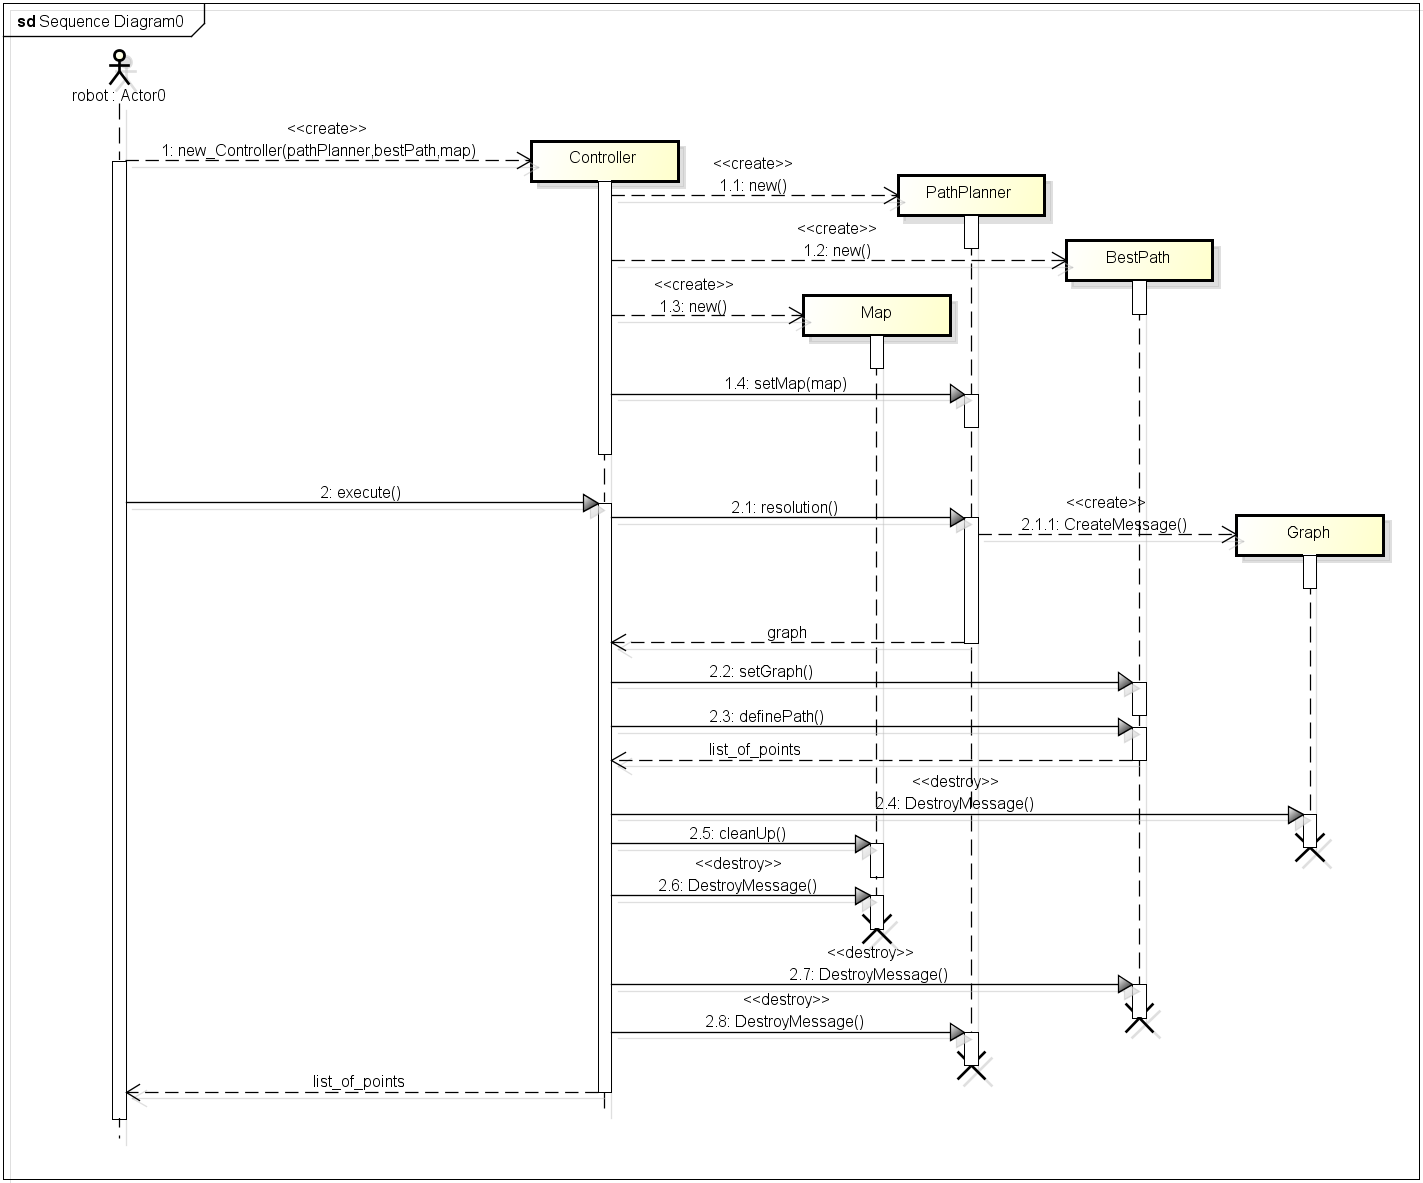
\includegraphics[keepaspectratio=true,scale=0.4]{figuras/executeController.png}
	\caption{Diagrama de sequência do componente controller}
\end{figure}

\subsection{Map}

\begin{figure}[h]
	\centering
	\label{fig27}
		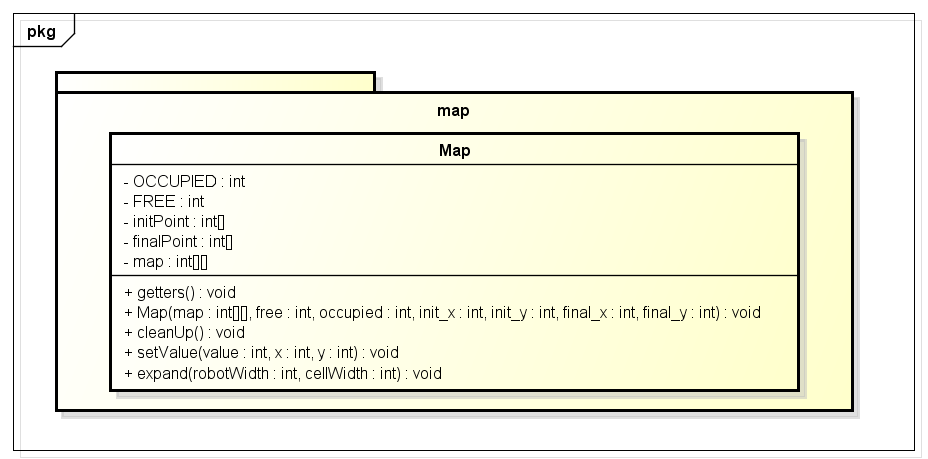
\includegraphics[keepaspectratio=true,scale=0.5]{figuras/pkgmap.png}
	\caption{Componente Map}
\end{figure}

O componente Map armazena a estrutura do mapa em seu interior. O componente recebe do controlador os dados das posições e guarda essa referência dentro de si para fazer as alterações necessárias. O objeto Map centraliza os dados que a camada de sensoriamento fornece e funções específicas da definição de trajetória que agem sobre eles, como: definir pontos inicial e final; conferir pesos às posições (células); expandir obstáculos, e diferenciar espaços livres de obstáculos.

Internamente, o mapa trabalhado é considerado uma matriz de inteiros, sendo convertido para esse formato logo no construtor da classe. Como esse módulo fica fora do robô, nenhuma alteração feita nos dados recebidos comprometerá os dados reais no robô. A Figura 27 mostra os principais atributos e métodos da classe.

\subsection{Path Planner}

\begin{figure}[h]
	\centering
	\label{fig28}
		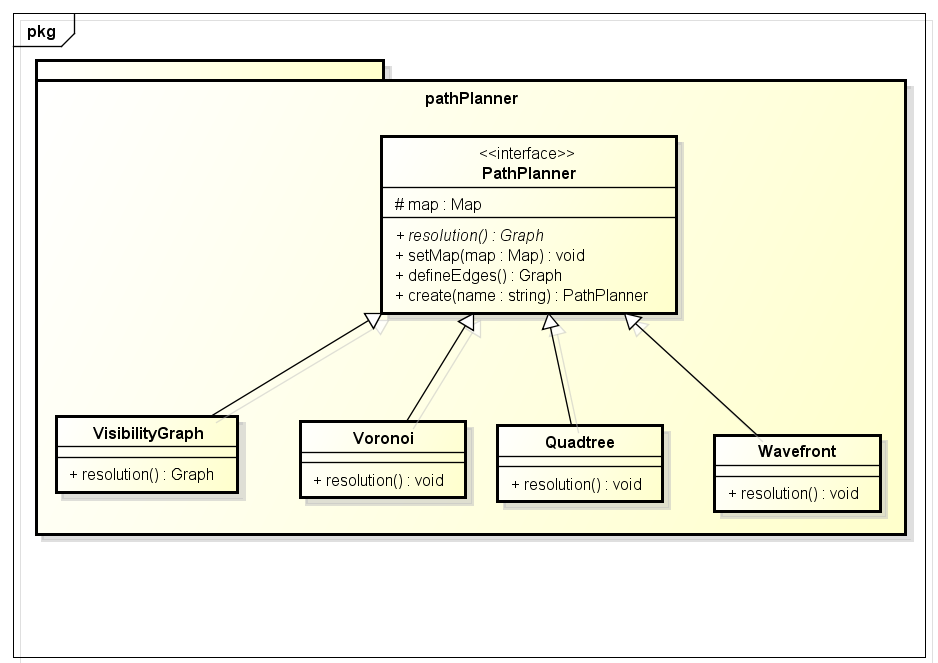
\includegraphics[keepaspectratio=true,scale=0.5]{figuras/pkgpathplanner.png}
	\caption{Componente PathPlanner}
\end{figure}

O PathPlanner é o componente responsável por implementar os algoritmos de definição de trajetória. A classe abstrata PathPlanner carrega funções úteis às classes concretas e fornece um método abstrato que deve realizar o algoritmo. Cada subclasse sobrescreve \textit{resolution} e métodos específicos e cria um grafo diferente. A classe abstrata também possui um método Fábrica para definir qual subclasse dele será utilizada. A Figura 28 mostra a classe abstrata e todas as classes concretas implementadas.

Graças à interface comum aos algoritmos é possível tratá-los de forma igual em todo o resto do sistema. O comportamento diferente entre eles (a criação do grafo) é abstraído para as subclasses, enquanto a superclasse se preocupa com o que for igual, definindo as entradas e saídas comuns. Isso segue o princípio de Variações Protegidas apresentado por \cite{Larman2005}, implementado através do padrão Strategy. O padrão Injeção de Dependência diminui seu acoplamento com o módulo Map, recebendo o mapa já pronto para trabalhar do controlador.

\subsection{Graph}

\begin{figure}[h]
	\centering
	\label{fig29}
		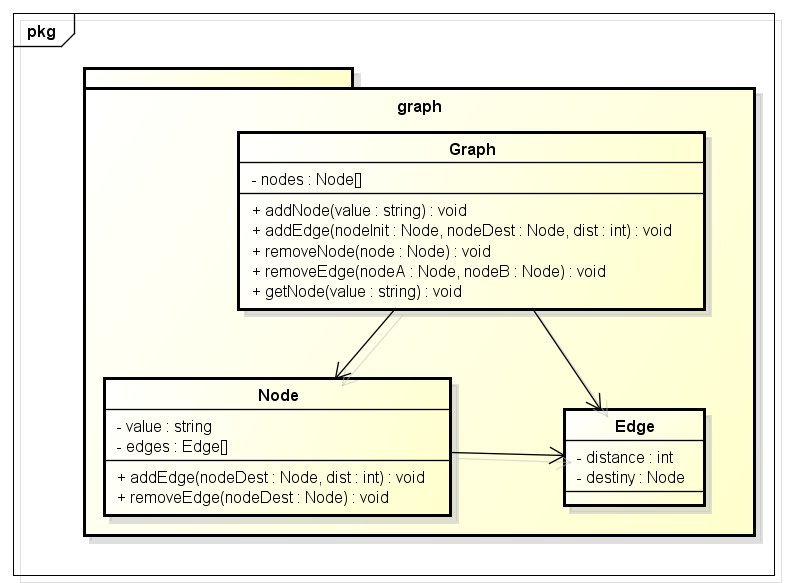
\includegraphics[keepaspectratio=true,scale=0.5]{figuras/pkggraph.png}
	\caption{Componente Graph}
\end{figure}

O módulo Graph é responsável por manter a estrutura do grafo. O grafo mantém uma lista de nós que representam pontos navegáveis no espaço. Cada nó possui uma lista de arestas (\textit{edges}) que o liga a outros nós.

A classe grafo possui métodos para a construção, busca e eliminação de nós e arestas, podendo realizar qualquer operação CRUD através do próprio objeto grafo ao invés de trabalhar diretamente em cada nó. A Figura 29 demonstra os métodos principais e a relação entre os mesmos.

\subsection{Best Path}

\begin{figure}[h]
	\centering
	\label{fig30}
		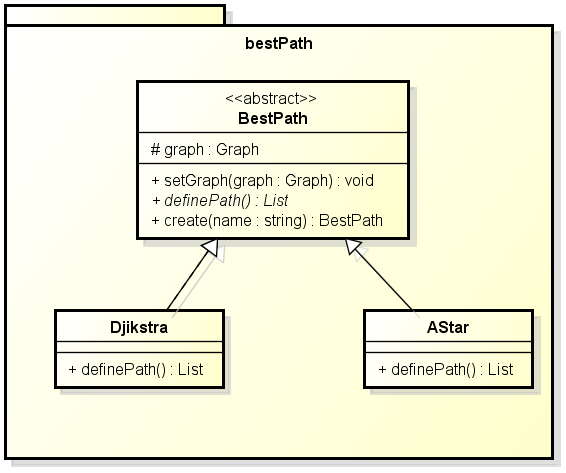
\includegraphics[keepaspectratio=true,scale=0.5]{figuras/pkgbestPath.png}
	\caption{Componente BestPath}
\end{figure}

O Best Path é o componente que define o melhor caminho a ser executado pelo robô. Recebendo o grafo com os pontos navegáveis, este módulo define um trajeto a partir de alguma característica desejada (ex. menor caminho, menor curvatura e outras). Esta carecterística é definida pela subclasse escolhida pelo usuário. No caso, as duas subclasses mostradas no diagrama definem o percurso por menor caminho, porém novas extensões podem ser criadas para formar o trajeto a partir de outra característica. A Figura 30 mostra as três classes desenvolvidas.

Novamente, a classe abstrata BestPath define as características comuns a todos os algoritmos, determinando as entradas e saídas que receberão. A implementaçao de como trabalhar com o grafo e criar a lista de pontos pelos quais o robô passará dependerá da implementação escolhida.

Assim como no componente pathPlanner, o princípio de Variações Protegidas é realizado através do padrão Strategy e a criação da classe é generalizada pelo padrão Fábrica.

\section{O Protótipo}

Para validação da ideia, foi desenvolvido um protótipo funcional que provasse a viabilidade do projeto. Nos primeiros meses de trabalho, foi modelada e implementada a arquitetura do \textit{framework} e desenvolvido o algoritmo Quadtree e Djikstra para testar todo o fluxo de execução da ferramenta. Além disto, foram também realizados os testes para as classes produzidas.

No protótipo, o \textit{framework} todo seria executado dentro do robô, assim não existia os módulos de comunicação \textit{bluetooth} e o código do robô instanciava diretamente as classes concretas dos \textit{hot-spots} desejados, sem necessidade de um método Fábrica. A figura 31 mostra um exemplo de como o Lejos chamava o Traveller.

\begin{figure}[h]
	\centering
	\label{fig31}
		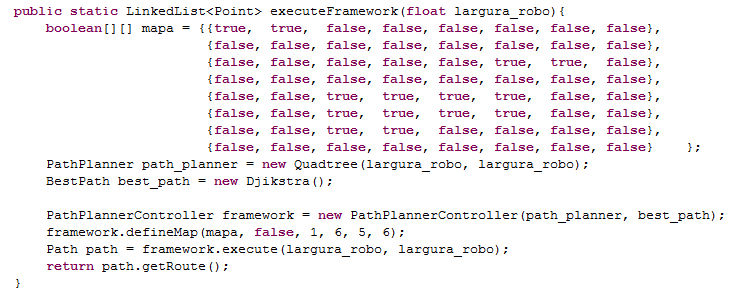
\includegraphics[keepaspectratio=true,scale=0.8]{figuras/codigoprototipo.PNG}
	\caption{Código do \textit{framework} sendo executado na versão protótipo}
\end{figure}

A arquitetura do protótipo era próxima da atual e já implementava a maioria das interfaces e padrões presentes na versão final. As maiores diferenças estavam no número de implementações de cada \textit{hot-spot} e na inexistência dos módulos web. De início, foi realizada uma análise sobre todo o projeto e foram levantados os \textit{hot-spots} \textit{PathPlanner} e \textit{BestPath}. 

A classe PathPlannerController tinha inicialmente como propósito servir de intermediário entre o usuário do \textit{framework} e as funções implementadas por ele. Essa era a classe principal do sistema em sua primeira versão, encapsulando todo o funcionamento e sendo chamada pelo usuário para realizar tudo. Isso mudou com o repasse ao servidor, mas a classe manteve sua função de gerenciar o fluxo de atividades.

A suíte de testes realizadas nessa primeira fase realizava testes unitários simples sobre o código, verificando se o grafo montado pelo Quadtree estava como esperado, verificando se todos os nós que deveriam existir foram criados. Os testes também verificaram o caminho gerado pelo Djikstra, ou seja, se era o mesmo que o esperado para aquele mapa. Sete mapas pequenos foram desenhados e, seus grafos e caminho a ser percorrido, calculados a mão para validar os algoritmos. Os mapas possuíam entre 4 e 9 casas de largura e comprimento, podendo ser perfeitamente quadrados ou retangulares.

\section{A Versão Final}

O código final trabalha como descrito na seção 5.1, permitindo a livre escolha entre algoritmo de melhor caminho e definição da trajetória. A interface no robô é a única camada que o usuário precisa conhecer e, caso ainda não haja uma implementação para sua plataforma, desenvolvê-la faz-se necessário.

O usuário precisará ainda baixar o código do lado servidor e rodá-lo em uma máquina próxima ao ambiente em que o robô trabalhará. Considerando que o Traveller trabalha com algoritmos globais e ambientes estáticos, o mesmo é recomendado apenas para ambientes fechados e bem conhecidos, como residências, escritórios ou fábricas. Nestes ambientes, um computador precisará ser instalado e com o Java e o \textit{framework} configurados. Será ainda preciso possuir comunicação \textit{blueooth} e que a mesma esteja habilitada.

A figura 32 mostra um exemplo de código embarcado no robô Lego NXT usando o Traveller.

\begin{figure}[h]
	\centering
	\label{fig32}
		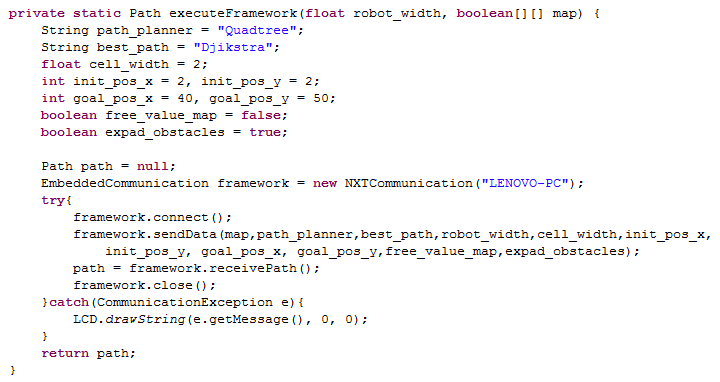
\includegraphics[keepaspectratio=true,scale=0.8]{figuras/codigofinal.PNG}
	\caption{Código do \textit{framework} sendo executado na versão final}
\end{figure}

A decisão de portá-lo para um servidor externo foi devido aos testes de memória e processamento realizados no mesmo, os quais serão apresentados em detalhes na seção 6.2. Outro resultado mostrado pelos testes de desempenho foi alto gasto de tempo com funções de acesso às listas presentes nas classes (\textit{get}). Em diversas partes do código, foram utilizadas listas encadeadas para armazenar dados. Uma das funções que mais consumia tempo no processador era a de recuperar um dado destas listas. Assim, outra alteração foi o tipo de estrutura utilizada para armazenar estes dados, trocando do \textit{LinkedList} para o \textit{ArrayList} (ambos fornecidos pelo Java).

Caso queira, o usuário pode alterar o comportamento dos algoritmos ou implementar novos que sejam compatíveis com o \textit{framework}, uma vez que possui o código fonte instalado em seu computador e o mesmo foi estruturado para isso. Foi escolhido realizar a implementação básica de cada algoritmo, por serem soluções clássicas em seus meios. Assim, versões otimizadas dos algoritmos como os propostos por \cite{Souza2008} e \cite{Medeiros2011} não foram implementadas. Entretanto, podem ser incluídas como outras classes filhas da classe abstrata.

Dos quatro algoritmos desenvolvidos, o algoritmo de Voronoi foi o único a apresentar falhas em seu resultado, realizando um percurso fora do esperado para o comportamento descrito no capítulo 2.4.2 e, na maioria das vezes, não conseguindo encontrar um percurso entre os pontos inicial e final. Todos os demais geram um grafo e devolvem uma lista de pontos compatível com o comportamento descrito no capítulo 2.4.

Além dos algoritmos implementados, outros foram estudados, bem como analisadas suas visibilidades. Um deles foi o algoritmo D* \cite{Ferguson__2005_5119} para definição de trajetória, porém não incluso por seu uso não se encaixar no cenário de algoritmos globais e do Traveller.

\section{\textit{Hot-spots} do \textit{Framework}}

Como definido pelo processo de produção de \textit{framework} de \cite{Fayad1999}, a análise de \textit{hot-spots} é algo iterativo, levantado ao longo da produção com apoio de um especialista. O Traveller possui ao todo três \textit{hot-spots}: \textit{PathPlanner}, \textit{BestPath} e \textit{EmbeddedCommunicator}. O usuário pode incrementar e configurar estes componentes, escolhendo entre as soluções já implementadas e inserindo novas. Seus \textit{hot-spots} servem de gancho para mudanças.

Para dar a variabilidade necessária nesses pontos, para a variância destes pontos foram utilizados os padrões de projeto descritos no tópico 5.1. Eles oferecem a flexibilidade para mudanças sem gerar impactos nos demais módulos, mantendo a coesão alta e o acoplamento baixo entre os módulos.

\subsection{PathPlanner}

Incluso desde a primeira versão do código, este é o principal \textit{hot-spot} do \textit{framework}, dando a liberdade de trocar entre os algoritmos de definição de trajetória. O padrão \textit{Strategy} fornece a variação sem impactos de manutenção no código, e o padrão Fábrica permite a instanciação da classe especificada pelo usuário. Como o núcleo do Traveller foi retirado de dentro do robô, o usuário não pode instanciar diretamente mais a versão desejada. Assim sendo, o padrão Fábrica permite a verificação do texto recebido pela rede, iniciando o objeto correto.

O \textit{hot-spot card} do \textit{PathPlanner} encontra-se no apêndice A.

\subsection{BestPath}

Também incluso desde a primeira versão, este módulo foi projetado de forma igual ao \textit{PathPlanner}. Ele recebe a saída do módulo \textit{PathPlanner} para gerar o resultado final do \textit{framework}, sendo assim parte do fluxo principal do mesmo. Suas classes concretas são escolhidas via Método Fábrica também e isolam a implementação na classe filha, permitindo que cada classe tenha seu próprio algoritmo. Isso permite que soluções bastante diferentes sejam chamadas com a mesma interface, como um algoritmo que retorne o menor caminho e outro que retorne o caminho mais suave.

O \textit{hot-spot card} do \textit{BestPath} encontra-se no apêndice A.

\subsection{EmbeddedCommunicator}

Este \textit{hot-spot} permite que robôs diferentes consigam conversar da mesma forma com o \textit{framework} no servidor. Isso é feito implementando a sequência de passos para a troca de mensagens com o servidor, passando os dados e as classes a serem instanciadas, e abstraindo a função de comunicação para as classes concretas. Cada classe filha fornece os métodos para enviar e receber dados para um \textit{hardware} diferente.

O \textit{hot-spot card} do \textit{EmbeddedCommunicator} encontra-se no apêndice A.

\subsection{\textit{Hot-spot} Descartados: O Mapa}

Durante boa parte do desenvolvimento do \textit{framework} imaginou-se que o mapa poderia vir a se tornar um \textit{hot-spot}. Permitir que o usuário use qualquer tipo de representação de mapa mostrada no capítulo 2.3 aumentaria o número de interessados no uso da ferramenta e a tornaria mais flexível. Essa questão foi profundamente analisada e chegou-se a construir seu \textit{hot-spot card}. Entretanto, a inclusão do \textit{hot-spot EmbeddedCommunicator} e a transferência do módulo Map para o servidor tornou o desenvolvimento desse \textit{hot-spot} mais complexo. 

Antes, uma solução semelhante a do \textit{BestPath} e \textit{PathPlanner} poderia ser utilizada, porém ao ter que passar os dados para o servidor se perderia sua estrutura atual, desconhecida até então pelo \textit{EmbeddedCommunicator}. Seria preciso uma estrutura genérica capaz de armazenar as informações de qualquer tipo de mapa sem perder seu sentido para então convertê-lo na matriz de inteiros. Outra solução seria converter o mapa para uma matriz de inteiros ainda no robô e já enviar ao servidor da forma desejada, porém Isto aumentaria o acoplamento entre as partes e consumiria muita memória do robô, que precisaria por alguns instantes guardar dois mapas na memória. Sendo assim, o \textit{hot-spot} \textit{Map} foi descartado desta versão final.

\section{Os Obstáculos}

Os obstáculos são representados por células de valores diferentes no mapa, marcando-as como ocupadas. Contudo, algumas considerações sobre os obstáculos precisam ser feitas independente da forma que são implementados esses obstáculos.

O robô é considerado como um ponto (seu centro), o que pode gerar problemas se ele se aproximar demais dos obstáculos. Um algoritmo considerando o robô um ponto pode fazê-lo passar muito perto do obstáculo achando que nada acontecerá. Entretanto, quando executado o algoritmo, a colisão ocorre. \cite{Guzman2008} diz que os algorítmos Grafo de Visibilidade e Quadtree passam o mais perto possível dos obstáculos, gerando um menor percurso, porém esse mais arriscado. Para evitar que esses algoritmos causem a colisão do robô com o obstáculo uma solução dada por \cite{Souza2008}, \cite{Guzman2008}, \cite{Siegwart2004} e \cite{Thomsen2010} é a expansão dos obstáculos. O algoritmo considera os obstáculos maiores do que realmente são, aumentando o obstáculo em, no mínimo, metade da largura do robô para que o centro passe tangente ao novo vértice sem haver real contato. Para isso, é preciso receber no controlador dois parâmetro a mais, o tamanho do robô e quanto mede cada célula do mapa. O controlador, então, determina quantas células o robô mede de largura e incrementa a metade mais um em todos os obstáculos.

\begin{figure}[h]
	\centering
	\label{fig33}
		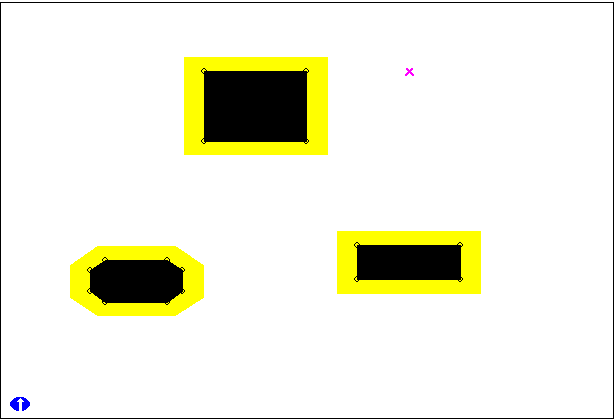
\includegraphics[keepaspectratio=true,scale=0.5]{figuras/expansao.png}
	\caption{Obstáculo real em preto e a expansão incrementada em amarelo \cite{MRIT_SITE}}
\end{figure}

Vale lembrar que esta expansão pode mudar o percurso do robô. Um percurso passando entre dois obstáculos pode ser fechado por este incremento. Isso impede que o robô entre em corredores muito estreitos ou entre em regiões côncavas de um obstáculo.

O Traveller permite a escolha da expansão ao não pelo usuário. A classe Map possui um atributo booleano que guarda se os obstáculos devem ou não ser expandidos. Por padrão, o \textit{framework} não expande. Ao expandir, o Traveller marca as células expandidas como ocupadas, sendo portanto, realizada a expansão apenas ao executar fluxo completo do \textit{framework}.

Outra consideração são os obstáculos côncavos. \cite{Siegwart2004} e \cite{Guzman2008} abordam a eliminação de pontos que formem áreas côncavas nos obstáculos. O simulador MRIT, citado também, segue esta abordagem. Outros autores como \cite{Thomsen2010} e \cite{Choset2005} não fazem esta consideração, pois nem sempre o espaço côncavo de um polígono é pequeno a ponto de ser perigoso e por vezes pode ser o único caminho até o objetivo. 

Computar os vértices côncavos, além de consumir maior tempo e aumentar a complexidade do algoritmo de detecção de vértices, torna o grafo muito maior. Com o maior número de pontos a serem considerados, os algoritmos que dependem dessa informação (grafo de visibilidade e Voronoi) tornam-se mais demorados e consomem mais memória. Desconsiderar estes pontos só impactam de forma decisiva sobre o percurso final se o mesmo for o menor caminho entre os pontos inicial e final e se a passagem que passa pela região côncava for estreita (próxima ao tamnho do robô). Considerando isso os pontos côncavos são desconsiderados pelo Traveller.

\section{Boas Práticas de Programação}

Não apenas escrever um código que funcione, é preocupação da engenharia de software que o código seja manutenível. Isso inclui, além da modularidade e uso de padrões conhecidos, escrever um código legível e simples. \cite{Goodliffe2007} e \cite{McConnel2004} descrevem características de um bom código e servem como um guia para boa programação.

Essas técnicas dão uma maior qualidade ao código, melhorando manutenibilidade, e aumentando a coesão e a reutilização. Tais temas são abordados pelos dois autores. As práticas sugeridas por eles não resolvem os problemas do sistema ou implementam suas funcionalidades, mas estão voltadas para a qualidade a longo prazo. Futuramente, a alteração e inserção de novas funcionalidades ao Traveller será facilitada com estas práticas, permitindo o crescimento do mesmo com menor esforço para sua compreensão.

Algumas dessas características, seguidas no desenvolvimento deste projeto, são:

\begin{itemize}
  \item \textbf{Testes inteligentes:} \cite{Goodliffe2007} e \cite{McConnel2004} enfatizam que testes devem ser sempre realizados. Sempre teste o código após fazê-lo, não deixando para outro momento. Eles também enfatizam que os testes devem ser focados nos princiais fluxos do sistema. Tentar testar todas as possibilidades do código é inviável e muitas delas raramente virão a ocorrer. Por isso, testes devem ser focados nas partes principais, rodando todos os fluxos das funcionalidades centrais do sistema, testando o \textit{design} do sistema para validá-lo como robusto e testando só os fluxos principais das características menos vitais do sistema. \cite{McConnel2004} sugere o uso de testes automatizados e de cobertura de código.
  \item \textbf{Manter o mesmo estilo de escrita:} o código deve manter o mesmo padrão de escrita por todo o sistema. Se as chaves usadas ao abrir um bloco de instrução estarão na mesma linha ou na de baixo, a identação, comentários, quebras de linha e outras variações devem ser padronizadas para facilitar a leitura e torná-lo mais agradável de ser lido.
  \item \textbf{Nomes significativos:} o leitor deve ser capaz de saber do que se trata a variável, método ou classe apenas lendo seu nome. O nome deve se referir ao comportamento, identidade ou padrão ao qual está relacionado. \cite{Goodliffe2007} afirma que se o programador não sabe qual nome dar a uma variável ou função é porque não sabe exatamente o que ela faz.
  \item \textbf{Testar as entradas do sistema:} Não confiar que os valores recebidos estão sempre corretos é indispensável para um código seguro. Deve-se sempre checar se os valores estão dentro da margem esperada e se objetos não são nulos. Isso vale não só para os dados vindos de fora do \textit{framework}, valores vindo de outras classes e módulos devem ser verificados para garantir que não está sendo recebido um objeto nulo e evitar falhas de segmentação.
  \item \textbf{Clareza sobre código curto:} é preferível que o código fique maior do que difícil de entender. Dividir equações em várias linhas, simplificar as linhas de algorítmos e deixar apenas uma operação por linha são algumas das ações para tornar o código limpo e legível.
  \item \textbf{Considerar casos excepcionais:} mesmo que uma possibilidade de valor seja rara o código deve está preparado para tratá-la. Um conjunto de \textit{if-else-if} em sequência deve sempre ter um bloco \textit{else} ao final para casos fora do esperado, assim como todo bloco \textit{switch} deve possuir uma cláusula \textit{default}. O programa deve estar pronto para criar o objeto incompleto ou lançar algum tipo de exceção nesses casos.
  \item \textbf{Cuidados com variáveis:} sempre inicializar uma variável ao criá-la para evitar ler lixo de memória é uma das ações que tornam o código mais seguro, bem como criar a variável apenas quando ela for útil torna o código mais legível.
  \item \textbf{Evidencie o fluxo padrão do sistema:} O fluxo principal deve ser sempre o primeiro em estruturas condicionais como \textit{if-else} e \textit{switch}. O leitor do código deve conseguir acompanhar o fluxo comum do código, sem procurar em uma série de opções nas estruturas condicionais qual é a correta.
  \item \textbf{Simplicidade sobre velocidade:} um código otimizado é mais complexo. Inserir camadas, indireção e linhas extras diminuem a velocidade do sistema, mas o tornam organizado. Serão otimizados apenas blocos de código que necessitem de velocidade. A não ser que seja essencial, deve ser dada prioridade à simplicidade em todo o sistema. Para saber se o código necessita de otimização será preciso testá-lo com uma entrada complexa para analisar o tempo de processamento. Espera-se que os algorítmos Grafo de Visibilidade e Voronoi possam se tornar lentos e, caso isto ocorra de fato, suas implementações serão revistas.
  \item \textbf{Funções atômicas:} cada método deve realizar apenas uma função. Funções pequenas e simples tornam o código maior, porém o deixam fácil de compreender.
  \item \textbf{Retorne apenas uma vez:} cada função deve ter apenas uma cláusula \textit{return}. Sempre que possível evitar retornar uma função antes de seu fim.
  \item \textbf{Restrinja valores possíveis:} não permitir que uma variável assuma valores que ela não deveria ter. Definir uma variável como \textit{unsigned}, \textit{const} ou \textit{enum} quando necessário.
  \item \textbf{Comentários que façam diferença:} um código deve ser o mais auto-explicativo possível. Quando um comportamento ou operação for complexo demais um comentário pode ajudar a entender o código. Comentários óbvios ou descrevendo o que o código faz por alto serão evitados. O comentário deve explicar o por que o código age daquele modo, não como.
\end{itemize} 

\section{Resumo do Capítulo}

Foi desenvolvido um \textit{framework} de definição de trajetória implementando algoritmos globais. Como não se comunicam diretamente com sensores e atuadores, seu desenvolvimento se torna mais indepedente dos aspectos físicos do robô. O \textit{framework} será externo ao robô, sendo executado em um servidor e receberá os dados do robô para a execução e devolverá ao mesmo a lista de pontos a serem percorridos.

O Traveller Framework possui três \textit{hot-spots} em que pode ser escolhido o algoritmo pelo usuário e que podem ser extendidos por outros programadores. Esses \textit{hot-spots} são o algoritmo de definição de trajetória (PathPlanner), o algoritmo de menor caminho (BestPath) e a comunicação do robô com o servidor (EmbeddedCommunicator). Estes \textit{hot-spots} podem ser herdados e configurados como desejar.

Internamente, o Traveller trabalha com um mapa do tipo malha de ocupação com valores inteiros. A comunicação do robô com o \textit{framework} se dará por uma classe dentro do robô, herdada de \textit{EmbeddedCommunicator}. Serão passados os pontos inicial e final para esta classe, além do mapa e de quais algoritmos deseja executar. O \textit{EmbeddedCommunicator} repassa as informações ao servidor que instanciará os objetos e executará o fluxo da resolução, presente na classe Controller.

O \textit{framework} tem sete componentes: \textit{Graph} (responsável pelo grafo), \textit{Controller} (controlador do sistema), \textit{Map} (responsável pelo mapa), \textit{PathPlanner} (algoritmo global), \textit{BestPath} (algoritmo de melhor caminho), \textit{EmbeddedCommunicator} (responsável pela comunicação no lado do robô) e \textit{RobotCommunication} (responsável pela comunicação no lado do servidor). O desenvolvimento de cada um deles é embasado em boas práticas de programação e voltado à clareza e à simplicidade do código.